\setchapterpreamble[u]{\margintoc}
\chapter{Conclusions}
\labch{conclusions}
\label{sec:conclusions}

In this dissertation, the fusion of visible, multispectral and infrared imagery has been solved to shape a multi-layer system. This approach was extended to 3D point clouds by projecting the previous information to very dense \acrshort{rgb} point clouds that were accurately reconstructed with photogrammetry. Hyperspectral data was, on the other hand, fused with visible information and projected to a 2.5D point cloud. The compression and real-time rendering of large hypercubes were similarly solved with a stack-based representation. Then, a \acrshort{lidar} simulator was proposed to avoid the cumbersome tasks related to processing remotely sensed data as well as the acquisition of prohibitive technology, such as \acrshort{lidar}. Therefore, this simulator enabled generating large \acrshort{tls} and \acrshort{als} with semantic annotations and intensity from procedural and static scenarios. Both the simulation and the fusion of real data were approached with \acrshort{gpgpu}, thus reducing considerably the response time, even outperforming commercial solutions. Finally, simulated and real data were successfully applied to several case studies, from the optimization of \acrshort{tls} planning to the identification of thermal anomalies and the classification of hyperspectral patches to distinguish grapevine varieties.

On a non-technical level, these last three years have considerably contributed to improving as a researcher. The work carried out has led to important results that have been published in top journals and conferences from the Remote Sensing field, while others are still under review. In addition, I have had the pleasure of contributing to other colleagues' work, and despite those publications not fitting in this dissertation, they have greatly contributed to broadening my knowledge of Computer Graphics in other fields which are not my main area of expertise. 

\section{Summary of contributions}

First, a methodology for \textbf{correcting and fusing images from multiple data sources} at the image level was described. The Enhanced Correlation Coefficient was proposed as it was highly suitable for remotely sensed images sensible to different wavelength intervals. It behaved surprisingly well over datasets with significant radiometric differences. This method was massively applied to match visible, multispectral and infrared datasets. Furthermore, this algorithm was checked to highlight both the efficiency and quality of results and it provided remarkable results for images of lower dimensionality, even being blurred. In fact, missing part of the image details as well as reducing the image size helped in reducing significantly the response time while not obtaining much worse results. 

The image-matching procedure represents the baseline work of the first part of this dissertation. From here, \textbf{the aligned images were projected into 3D point clouds}. The advantages of working with point clouds rather than images are clear. For instance, they are better for visualizing a scenario at one glance, and location awareness is enhanced for human operators. However, point clouds are not as helpful if they are sparse or have geometrical errors. Therefore, a formal framework was presented for the generation of point clouds comprising visible, thermal and multispectral data. First, an \acrshort{rgb} point cloud was reconstructed using photogrammetry, typically with hundreds of millions of points and a high point density. The rest of the datasets were projected into this \acrshort{rgb} point cloud, thus tackling most of the drawbacks derived from applying photogrammetry over low-resolution imagery, e.g., thermal and multispectral. Additionally, this methodology outperformed commercial software in terms of 1) response time, 2) density and 3) size. Other considerations were to build an occlusion-aware projection using $z$-buffers and to optimize the aggregation of multiple image samples with aggregation and penalty functions. Following this approach, the aggregated radiometric data minimized the dissimilarity between the result and the initial samples. 

Furthermore, this pipeline was implemented in the \textbf{\acrshort{gpu}} to establish a fair comparison with commercial software such as Agisoft Metashape and Pix4Dmapper. Yet, the proposed methodology outperformed these commercial solutions in terms of response time. Other enhancements were checked, such as the global and local sorting of the point clouds. The conducted tests showed that globally reordering the point cloud significantly improved the response time, despite adding the latency from sorting. On the other hand, the global sorting followed by the shuffling of small groups, albeit promising, did not achieve better results for large point clouds due to the sorting overhead. 

The following step was to construct \textbf{hyperspectral point clouds}, which to the best of our knowledge had not been achieved before, at least not out of a laboratory. Hyperspectral swaths were fused with visible point clouds with a different pipeline adapted to the particularities of push broom sensors. The geometrical distortions were corrected by matching swaths with an \acrshort{rgb} orthomosaic, and then, a hyperspectral orthomosaic was composed by, again, minimizing the dissimilarity of the aggregated value and the starting collection of data. Then, this orthomosaic was projected into a 2.5D point cloud which was voxelized according to the hyperspectral \acrshort{gsd}. The large volume of the resulting hypercube was compressed with a stack-based representation in the radiometric dimension. However, this approach also led to a higher response time during rendering because of the iterative logic implemented in \textit{shaders}, especially for shading the last layers. This shortcoming was alleviated by constructing the images in multiple frames. In a similar way to previous work, the whole pipeline was implemented with \acrshort{gpgpu} and therefore it was proven to be very efficient.

The tedious task of acquiring, processing and including additional data in real-world datasets was partially avoided by generating synthetic \acrshort{lidar} data. \textbf{The \acrshort{lidar} technology was simulated} with the \acrshort{tof} principle plus systematic and random errors described in the literature. Atmospheric particles, highly reflective surfaces or slope- and height-derived errors were emulated. In addition, the sensor was parameterized to cover a wide range of commercial sensors through their specifications. Another key factor was the generation of procedural environments intended for scanning a large number of different environments and therefore, constructing large \acrshort{lidar} datasets. Scenes were first labelled and linked to materials according to name patterns that facilitate this manual task. Note that this task is only performed once in procedural scenes that are later composed following pre-defined instancing rules. Then, a comparison was established on the estimation of intensity in the returns: it was first modelled with traditional shading \acrshort{brdf}s, and then, these were simulated using \acrshort{brdf} databases comprising measurements obtained from a gonio-photometer. The comparisons showed that the obtained intensity histograms were similar, whereas the latter approach is more efficient and physically accurate, at the expense of having a larger memory footprint. Nevertheless, the volume of data was considerably reduced by assuming that \acrshort{lidar}'s emitter and receiver had the same position. The simulation was implemented in the \acrshort{gpu}, from the generation of \acrshort{lidar} beams to scanning, to rapidly solve aerial and terrestrial surveys. 

Unlike previous work, the proposed simulator includes \textbf{terrestrial and aerial surveys}, where the latter has barely been addressed. The path followed by both terrestrial and airborne vehicles can be defined, though it is especially relevant for \acrshort{als}, where paths are either user-defined or automatically calculated. Airborne surveys also required the simulation of different scanning patterns, from which parallel, zigzag and elliptical patterns stand out. The implementation of multiple returns was also relevant to simulate the filtering of canopy and vegetation to construct \acrshort{dem}s from airborne missions. Similarly, bathymetric \acrshort{lidar}s was also covered to scan shallow underwater areas. 

Datasets and results from previous chapters were utilized in practical case studies. First, the previous \acrshort{lidar} simulation helped in the \textbf{planning for scanning at indoor scenes}, using metaheuristics guided by objective functions. These evaluation functions were designed to maximize the number of intersected triangles, minimize the number of required scans and provide a dense point cloud. In addition, they do not require the user to intervene as most of the parameters are calculated as part of the pre-processing stage. Then, \textbf{thermal maps and point clouds were applied to inspect an archaeological site}, where two anomalous areas that may correspond to buried towers were spotted. Finally, \textbf{a hyperspectral dataset was applied to the classification of grapevine varieties}. Traditional techniques, based on the correlation of spectral signatures, did not fit well on the classification of very similar spectral signatures. Instead, a Deep Learning network was explored for the classification of grapevine varieties, using state-of-the-art layers such as Inception or spatial attention. The hyperspectral swaths were radiometrically corrected and transformed to have a lower number of features with Factor Analysis. Then, these were split into patches with a size tuned during experimentation, and reduced to a single label; hence, the classification of samples was influenced by its neighbourhood. Not only this network was proven to perform well over \acrshort{uas} datasets, but it also was able to obtain results close to the the-start-of-the-art overall accuracy in satellite imagery.  

\section{Future work}

Remote sensing and Deep Learning fields are rapidly evolving, and yet, there exist some future investigations that should be explored from this work:
\begin{itemize}
    \item Image matching was performed using commodity hardware, and therefore, it was explored whether downscaling and blur led to better response time. Indeed, it offered similar results with lower latency. From here, it could be explored if a pyramid scheme, from lower to higher size, helps to obtain better results while yet obtaining a low latency (see Figure \ref{fig:image_pyramid}). This way, larger transformations are computed from low-resolution imagery, whereas the most fine-grained changes are calculated with the starting dimensions. Besides reducing the response time, this approach could also help to match images with more notable differences.
    \begin{figure}
        \centering
        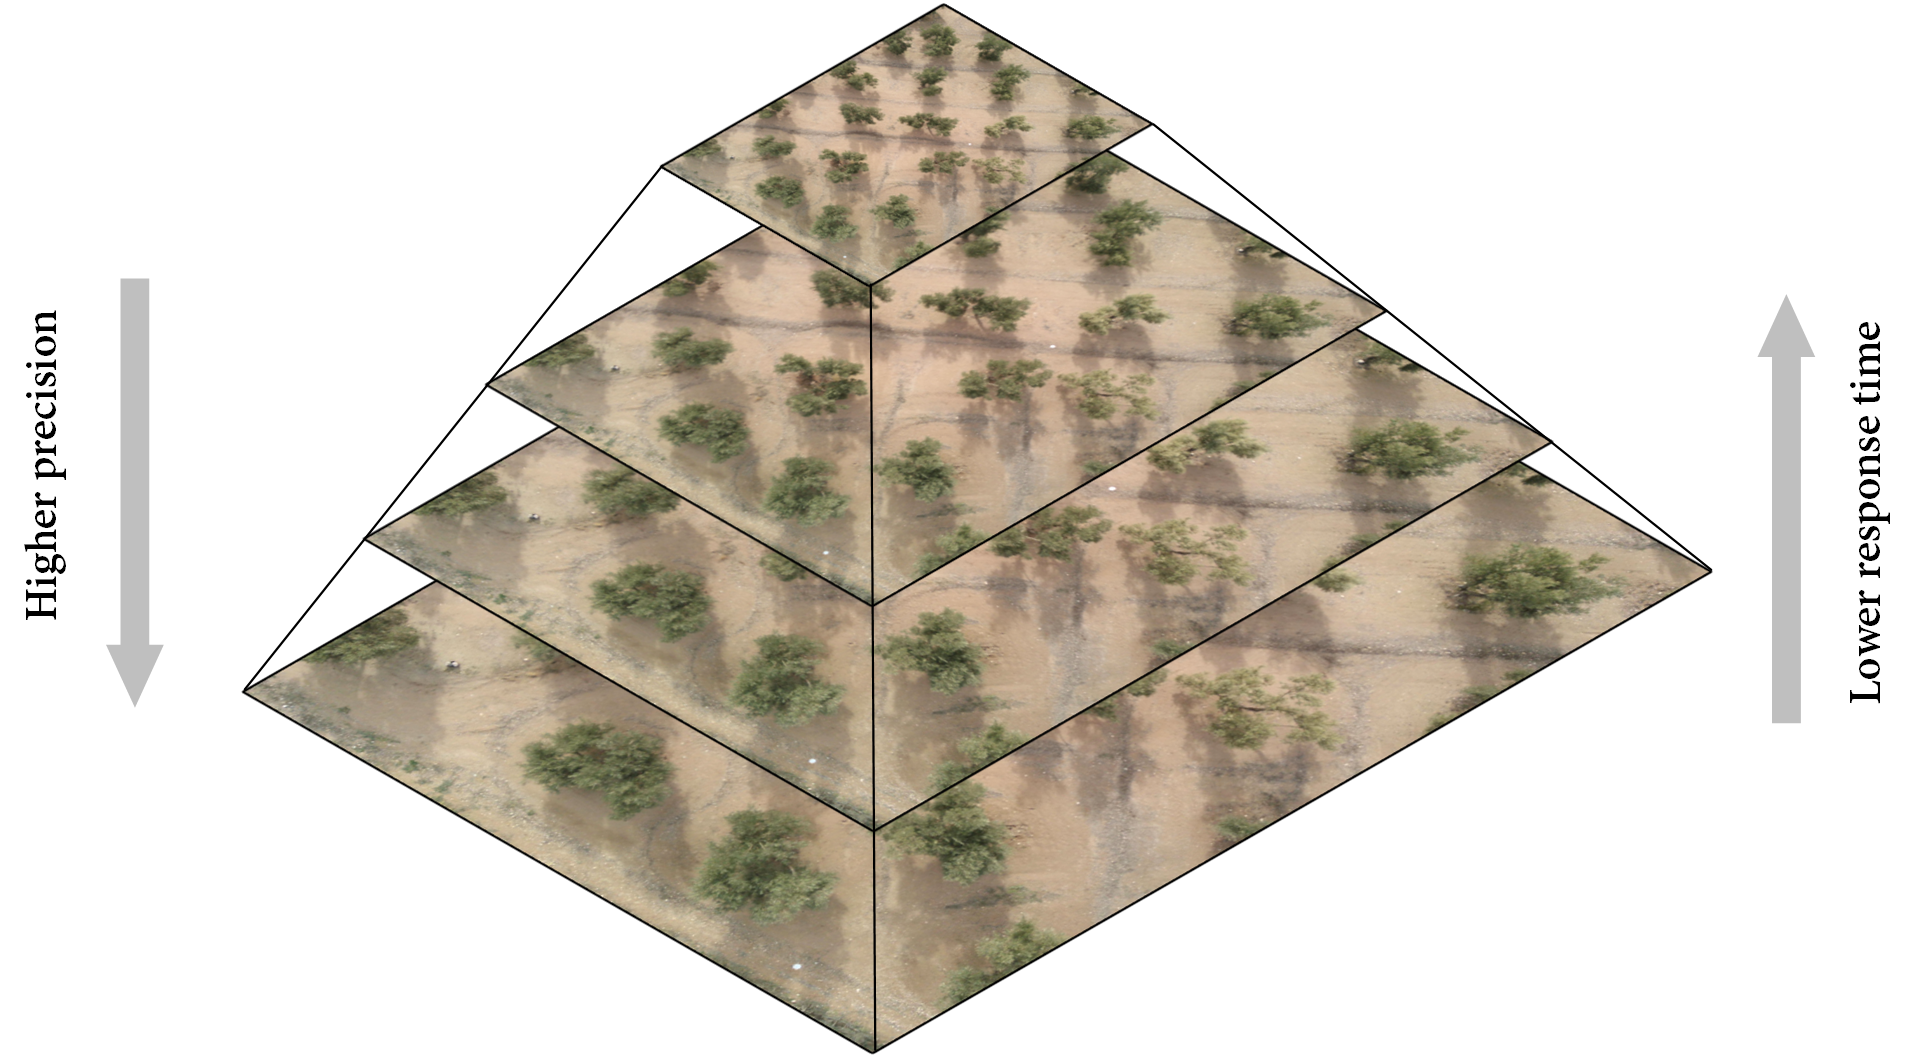
\includegraphics[width=\linewidth]{figs/conclusions/image_pyramid.png}
        \caption{Overview of an iterative image-matching algorithm, with higher image dimensionality providing slower but more fine-grained transformations.}
        \label{fig:image_pyramid}
    \end{figure}
    \item Image-matching was included as part of the reading phase in the comparisons established with commercial photogrammetry software. Therefore, this stage can be further accelerated by transferring the \acrshort{ecc} algorithm, currently obtained from OpenCV, to the \acrshort{gpu}.
    \item The generation of dense and large visible, thermal and multispectral point clouds helps to better visualize the scenario; however, point clouds with such a dimensionality are also harder to render in real-time. Although the compute-shader rendering alleviated this drawback \cite{schutz_rendering_2021}, it could be further enhanced with different levels of detail (\acrshort{lod}) \cite{schutz_gpu-accelerated_2023}. Similarly, it could help in the rendering of compressed hypercubes, since we already had to expand its real-time rendering over a few frames until completion.
    % \item The compression of hypercubes was achieved by lowering the radiometric resolution with a stack-based representation, whereas spatial compression was not possible since surrounding stacks were very different. Rather than a stack-based representation, compression could be achieved in the spatial dimension, which is known to be way larger than the spectral one. 
    \item \acrshort{lidar} optimization was studied as the simplest case study: a set of optimal locations that help to survey a scene with \acrshort{tls}. However, there are other kinds of \acrshort{lidar} which may be worth exploring, such as those that rely on a path rather than a set of locations. Swarm-based optimizations may fit better if a path is required \cite{roberge_fast_2018}. Optimization of airborne \acrshort{lidar} could also be explored to determine which is the optimal configuration to densely scan a scene from a \acrshort{dsm}, including, but not limited to the followed path.
    \item A similar approach to the latter proposal is to assess \acrshort{uas} missions by computing a path that guarantees the required overlap or coverage according to the time, altitude and \acrshort{uas} flight speed, among other factors. This has been achieved for generic \acrshort{uas} missions \cite{pessacg_simplifying_2022}, though it could be further improved based on the scene geometry, represented by rapidly sketched models. It could be especially relevant for oblique view directions, by setting it as an optimizable parameter rather than a user-defined factor. 
    \item So far, the \acrshort{lidar} simulations have helped to generate large \acrshort{lidar} datasets. However, there still remain some experiments that ought to be carried out to check whether these datasets are helpful for Deep Learning tasks. Note that some of the simulated errors will be filtered out once the point clouds are voxelized, which is the most widespread approach for feeding \acrshort{lidar} datasets \cite{hackel_semantic3d_2017, behley_towards_2021}. However, it should be discerned if these synthetic datasets are similar enough to the point distribution generated by real sensors. 
    \item Part IV addressed only the simulation of \acrshort{lidar} sensors. However, other sensors can be simulated by means of synthetically generated imagery. Generative Adversarial Networks (\acrshort{gan}), such as the one depicted in Figure \ref{fig:conclusions_gan}, have been gaining interest as they allow building computer-made unsupervised datasets. For instance, infrared data could be simulated from visible imagery to create larger datasets. The current state-of-the-art has not successfully achieved this task by learning solely from visible data \cite{li_multi-branch_2019, li_i-gans_2021, kniaz_thermalgan_2019, ozkanoglu_infragan_2022, yi_cycle_2023}, since it may require further information to isolate surfaces that have different radiance. 
    \item The phenotyping of grapevine varieties was approached with Deep Learning; however, this model could be improved by further integrating more varieties and collecting datasets at different stages of the year. Also, there are other interesting approaches to address this very same task, from multi-instance \cite{meerdink_multitarget_2022} to contrastive learning \cite{guan_spatial-spectral_2022}. 
\end{itemize}

\begin{figure}[H]
    \centering
    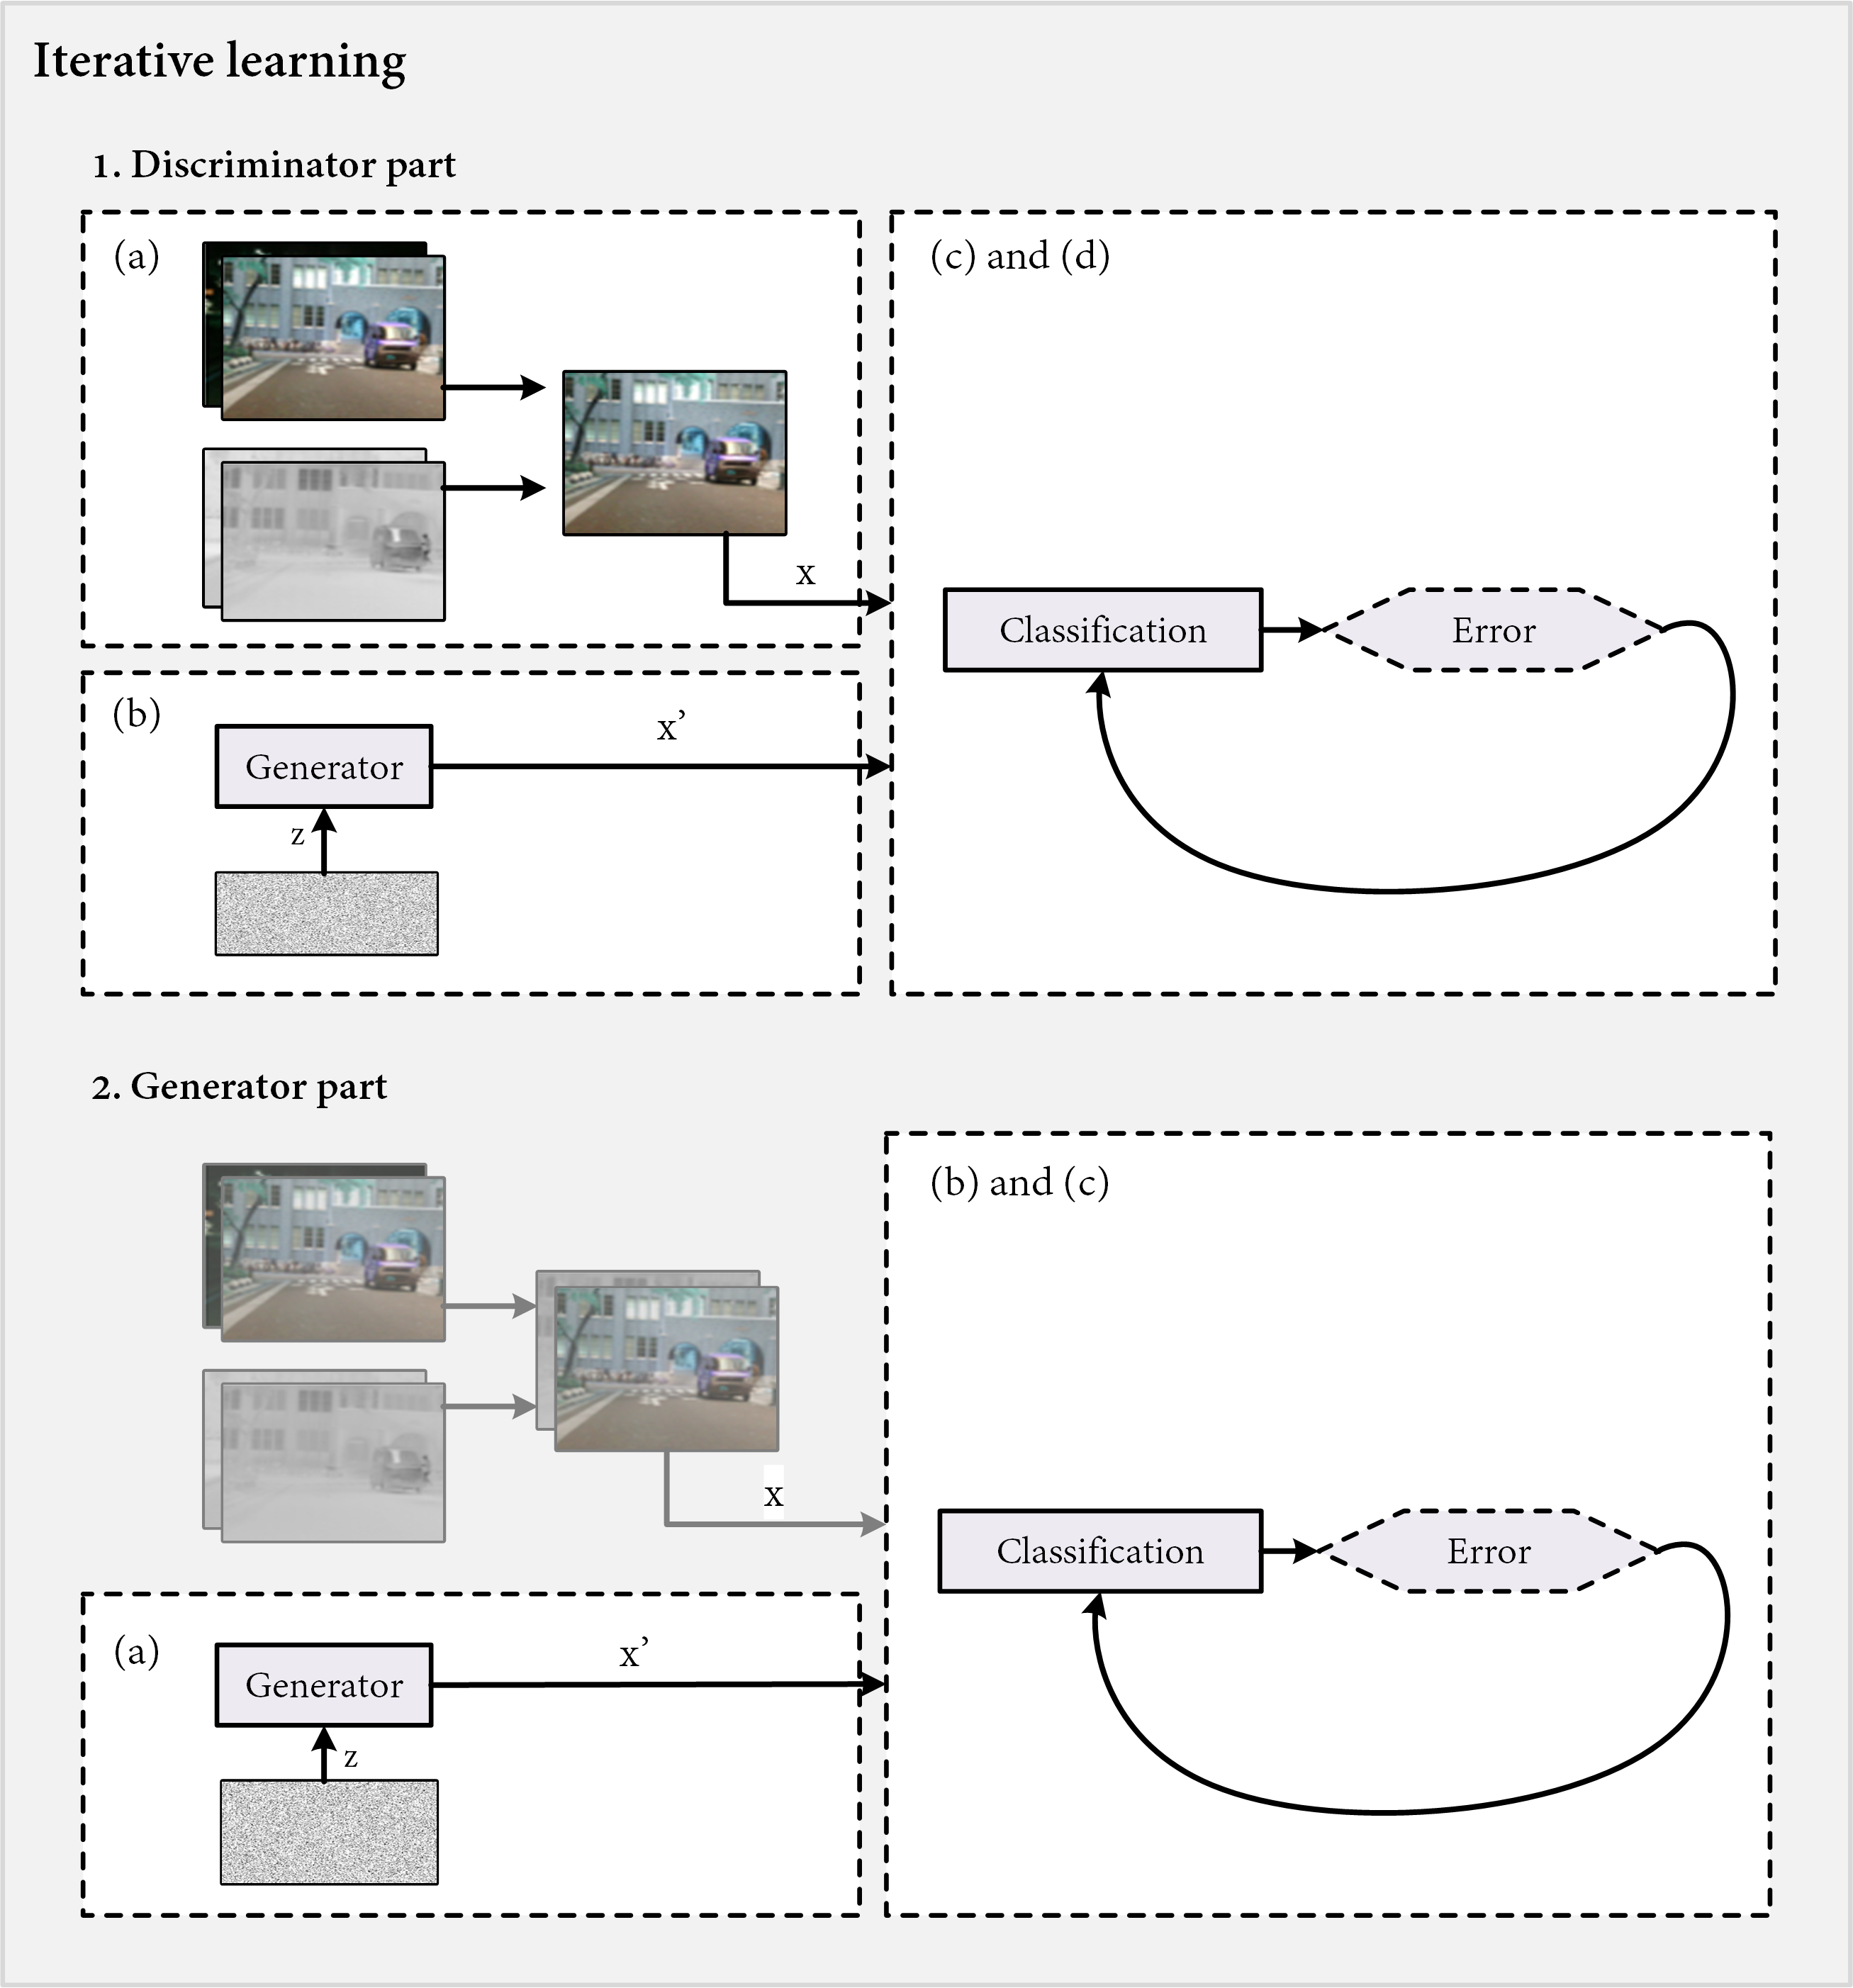
\includegraphics[width=\linewidth]{figs/conclusions/gan.png}
    \caption{Overview of a Generative Adversarial Network composed of discriminator and generator modules. The generator is trained to produce realistic data as similar as possible to the input data, while the discriminator is trained to distinguish between real and generated data.}
    \label{fig:conclusions_gan}
\end{figure}